\mode*
\begin{frame}
 	\section{Experimental Results}
 	\frametitle{Experimental Results}
 	\onslide<+->
	\textbf{Approaches and Settings}
	\begin{itemize}
		\item<+-> k-Nearest Neighbors
		\item<+-> Na\"ive Bayes
		\item<+-> Decision Tree
		\item<+-> Neural Network
		\item<+-> Ensemble
	\end{itemize}
\end{frame}

\begin{frame}
	\frametitle{k-Nearest Neighbors}
	\onslide<+->
	\begin{itemize}
		\item<+-> parameter search on a leave-one-out cross validation
		\item<+-> k=30 best (accuracy)
		\item<+-> distance measure = euclidean distance
		\item<+-> no distance weighting => better results
	\end{itemize}
\end{frame}

\begin{frame}
	\frametitle{Na\"ive Bayes}
	Another approach is the Na\"ive Bayes classifier. Despite some
	attributes obviously not being independent, it was still employed
	because it proved to be useful in other areas as well.
\end{frame}

\begin{frame}[fragile]
	\frametitle{Decision Tree}
	\onslide<+->
	\begin{itemize}
		\item<+-> prunes J48-decision tree
		\item<+-> confidence factor =  \(c=0.045\)
		\item<+-> found by utilizing WEKAs capabilities of linear
		parameter search
	\end{itemize}
\end{frame}

\begin{frame}[fragile]
	\frametitle{Neural Network}
	\onslide<+->
	\begin{itemize}
		\item<+-> multilayer perceptron
		\item<+-> 13 input neurons (features)
		\item<+-> hidden layer of 17 neurons
		\item<+-> output layer with three neurons (classes)
		\item<+-> learning rate: \(\alpha=0.1\)
		\item<+-> momentum:  \(m=0.1\) (backpropagation algorithm)
		\item<+-> linear search for parameters: hidden neurons, learning rate and momentum
	\end{itemize}
\end{frame}

\begin{frame}
	\frametitle{Ensemble}
	\onslide<+->
	\begin{itemize}
		\item<+-> Combine all models into an ensemble
		\item<+-> should combine the strength of the different classifiers
		\item<+-> ensemble was found by conducting a majority voting
	\end{itemize}
\end{frame}


\begin{frame}
	\frametitle{Results}
	\begin{itemize}
		\item 10-fold cross validation
	\end{itemize}
	\begin{figure}[h]
		\centering
		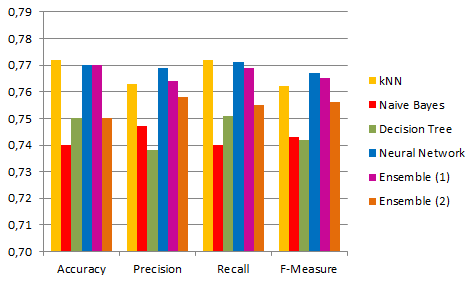
\includegraphics[width=0.7\columnwidth]{../../charts/results.png}
		\caption{Evaluation metrics of the different classifiers}
		\label{fig:result}
	\end{figure}
\end{frame}

\begin{frame}
	\begin{table}[h]
		\centering
		\caption{Confusion matrix of the ensemble}
		\label{tab:mat-vote}
		\resizebox{\columnwidth}{!}{
			\begin{tabular}[c]{c|ccc||c}
				classified \(\rightarrow\) & \textbf{Low} & \textbf{Medium} & \textbf{High} & Total\\ \hline
				Low & \textcolor{blue}{1125} & 126 & 8 & 1259 \\
				Medium & 160 & \textcolor{blue}{305} & 57 & 522 \\
				High & 15 & 95 & \textcolor{blue}{103} & 213 \\ \hline \hline
				Total & 1300 & 526 & 168 & 1994 \\
			\end{tabular}
		}
	\end{table}
\end{frame}


\begin{frame}
	\frametitle{Recall}	
	\begin{figure}[h]
		\centering
		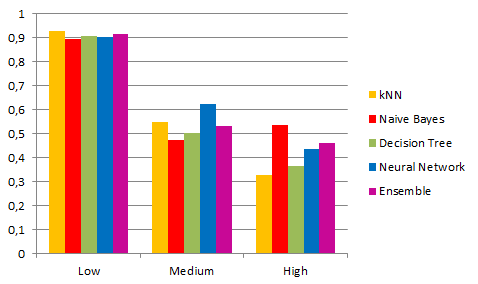
\includegraphics[width=0.7\columnwidth]{../../charts/recall.png}
		\caption{Recall of the different classifiers}
		\label{fig:recall}
	\end{figure}
\end{frame}
\mode<all>